\documentclass[12pt,a4paper]{article}
\usepackage[utf8]{inputenc}
\usepackage{graphicx}
\usepackage{float}
\usepackage{booktabs}
\usepackage{amsmath}
\usepackage{natbib}

\title{Analysis of Same-Side Bias in Coin Flipping}
\author{Wenqing Liu \and Evgenii Tishchenko}
\date{\today}

\begin{document}
\maketitle

\section{Introduction}
This study investigates the presence of same-side bias in coin flipping experiments, examining whether the outcome of a coin flip is truly random or influenced by systematic factors. We analyze data from multiple participants across different groups, considering various factors such as individual flipping techniques, coin characteristics, and potential learning effects.

\section{Exploratory Data Analysis}
Based on the distributions shown in Figure \ref{fig:person-group}, we analyze the results from two perspectives:

\textbf{Participant-level Analysis (Left Panel):}
\begin{itemize}
    \item \textbf{JanYang} and \textbf{TianqiPeng} show medians that notably deviate from the 0.5 baseline
    \item While other participants' medians remain close to 0.5, considerable within-participant variability exists
    \item Multiple outliers across participants suggest anomalous participant-coin combinations
\end{itemize}

\textbf{Group-level Analysis (Right Panel):}
\begin{itemize}
    \item All three groups (bachelor, internet, and marathon) show medians around the 0.5 baseline
    \item The marathon group shows greater dispersion, likely due to its larger sample size
    \item Bachelor and internet groups display more concentrated distributions
\end{itemize}

\subsection{Learning Effects}
\begin{figure}[h!]
    \centering
    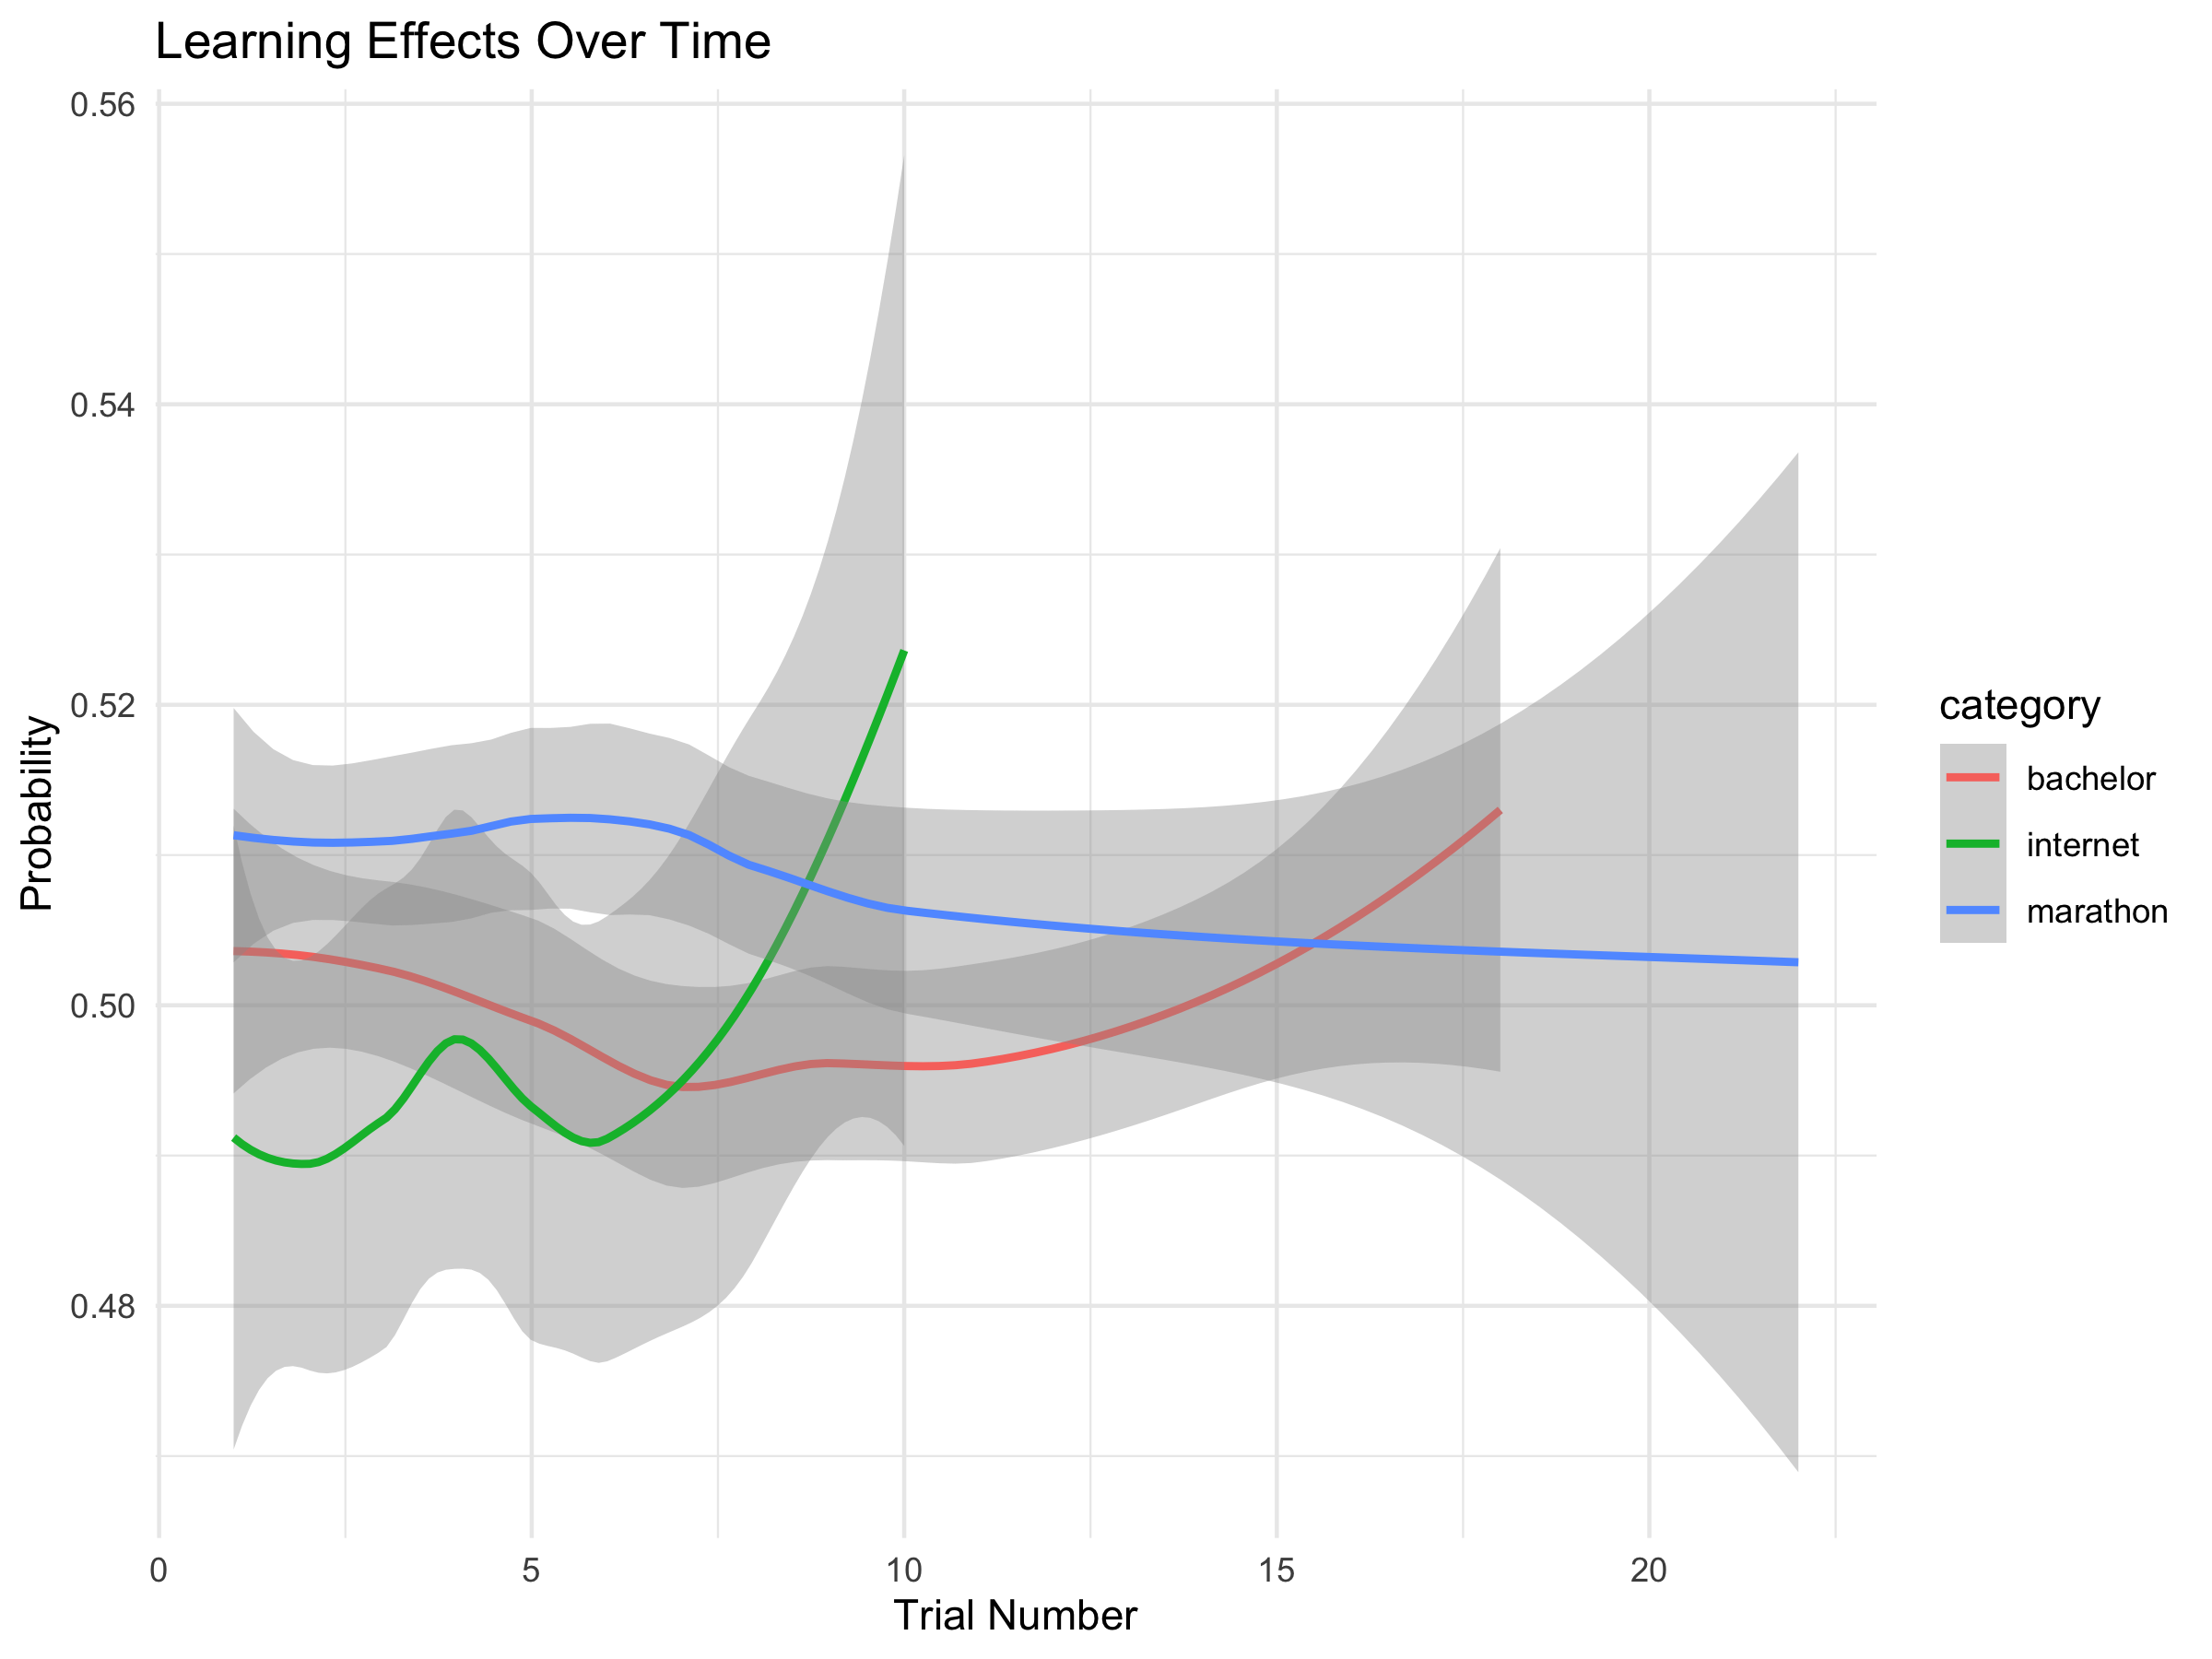
\includegraphics[width=0.8\linewidth]{learning_effects.png}
    \caption{Learning Effects Over Time by Group}
    \label{fig:learning}
\end{figure}

Figure \ref{fig:learning} shows the evolution of same-side probability over successive trials. The analysis reveals:
\begin{itemize}
    \item No strong systematic learning effects across groups
    \item Slight variations in early trials that stabilize over time
    \item Consistent group-level differences maintained throughout the experiment
\end{itemize}

\subsection{Coin Effects}
\begin{figure}[h!]
    \centering
    \includegraphics[width=0.8\linewidth]{coin_effects.png}
    \caption{Mean Same-Side Probability by Coin Type}
    \label{fig:coin-effects}
\end{figure}

Figure \ref{fig:coin-effects} illustrates the variation in same-side probability across different coin types, revealing:
\begin{itemize}
    \item Substantial variation between coin types
    \item Some coins consistently showing higher or lower same-side probabilities
    \item Error bars indicating the precision of estimates varies with sample size
\end{itemize}

\section{Methodology}
\subsection{Model Specification}
Following \cite{gelman2006data}, we employ a hierarchical modeling approach with stepwise model comparison. We start with the simplest model and gradually add complexity, evaluating the improvement in model fit at each step.

\subsubsection{Model Hierarchy}
We consider the following sequence of models:

\begin{enumerate}
    \item \textbf{Model 1 (Baseline)}: Intercept only
    \[
    \log\left(\frac{p}{1-p}\right) = \beta_0 + \epsilon
    \]
    
    \item \textbf{Model 2}: Adding participant random effects
    \[
    \log\left(\frac{p}{1-p}\right) = \beta_0 + u_i + \epsilon
    \]
    where $u_i \sim N(0, \sigma^2_u)$ represents participant-specific random effects.
    
    \item \textbf{Model 3}: Adding group fixed effects
    \[
    \log\left(\frac{p}{1-p}\right) = \beta_0 + u_i + \mathbf{X}_g\boldsymbol{\beta}_g + \epsilon
    \]
    where $\mathbf{X}_g$ represents group indicators.
    
    \item \textbf{Model 4}: Adding coin random effects
    \[
    \log\left(\frac{p}{1-p}\right) = \beta_0 + u_i + v_j + \mathbf{X}_g\boldsymbol{\beta}_g + \epsilon
    \]
    where $v_j \sim N(0, \sigma^2_v)$ represents coin-specific random effects.
    
    \item \textbf{Model 5}: Adding learning effects
    \[
    \log\left(\frac{p}{1-p}\right) = \beta_0 + u_i + v_j + \mathbf{X}_g\boldsymbol{\beta}_g + f(t) + \epsilon
    \]
    where $f(t)$ is a smooth function of trial number.
\end{enumerate}

\section{Results}
\subsection{Model Comparison}
We employed two different modeling approaches to analyze the same-side bias in coin flipping: Generalized Linear Mixed Models (GLMM) and Weighted Least Squares (WLS).

\subsubsection{GLMM Results}
\begin{table}[H]
\centering
\begin{tabular}{llrrr}
\toprule
\textbf{Model} & \textbf{Added Effects} & \textbf{AIC} & \textbf{BIC} & \textbf{Deviance} \\ 
\midrule
GLMM1 & Baseline & 3477.63 & 3485.72 & 433.98 \\
GLMM2 & + Group & 3478.44 & 3494.62 & 435.37 \\
GLMM3 & + Coin RE & 3479.50 & 3499.72 & 419.77 \\
GLMM4 & + Learning & 3480.93 & 3505.20 & 419.19 \\
\bottomrule
\end{tabular}
\caption{GLMM Model Comparison Results. RE = Random Effects}
\label{tab:glmm_comparison}
\end{table}

\subsubsection{WLS Results}
\begin{table}[H]
\centering
\begin{tabular}{llrrr}
\toprule
\textbf{Model} & \textbf{Added Effects} & \textbf{AIC} & \textbf{BIC} & \textbf{Adj. R²} \\ 
\midrule
WLS1 & Baseline & -727.90 & -719.81 & 0.000 \\
WLS2 & + Group & -738.01 & -721.83 & 0.028 \\
WLS3 & + Person & -838.34 & -640.14 & 0.307 \\
WLS4 & + Learning & -837.06 & -634.81 & 0.306 \\
\bottomrule
\end{tabular}
\caption{WLS Model Comparison Results}
\label{tab:wls_comparison}
\end{table}

\subsection{Model Selection and Parameter Estimates}
Based on the model comparison results, we can draw the following conclusions:

\begin{itemize}
    \item \textbf{GLMM Analysis}:
    \begin{itemize}
        \item The baseline model (GLMM1) shows the best BIC value, suggesting that more complex models may be overfitting
        \item Adding coin random effects (GLMM3) significantly reduces deviance but increases model complexity
        \item The addition of learning effects (GLMM4) does not provide significant improvement
    \end{itemize}
    
    \item \textbf{WLS Analysis}:
    \begin{itemize}
        \item Including person effects (WLS3) significantly improves model fit, explaining approximately 30.7\% of variance
        \item Adding learning effects (WLS4) provides no additional explanatory power
        \item Group effects are relatively small, explaining only about 2.8\% of variance
    \end{itemize}
\end{itemize}

\subsection{Random Effects Analysis}
\begin{figure}[h!]
    \centering
    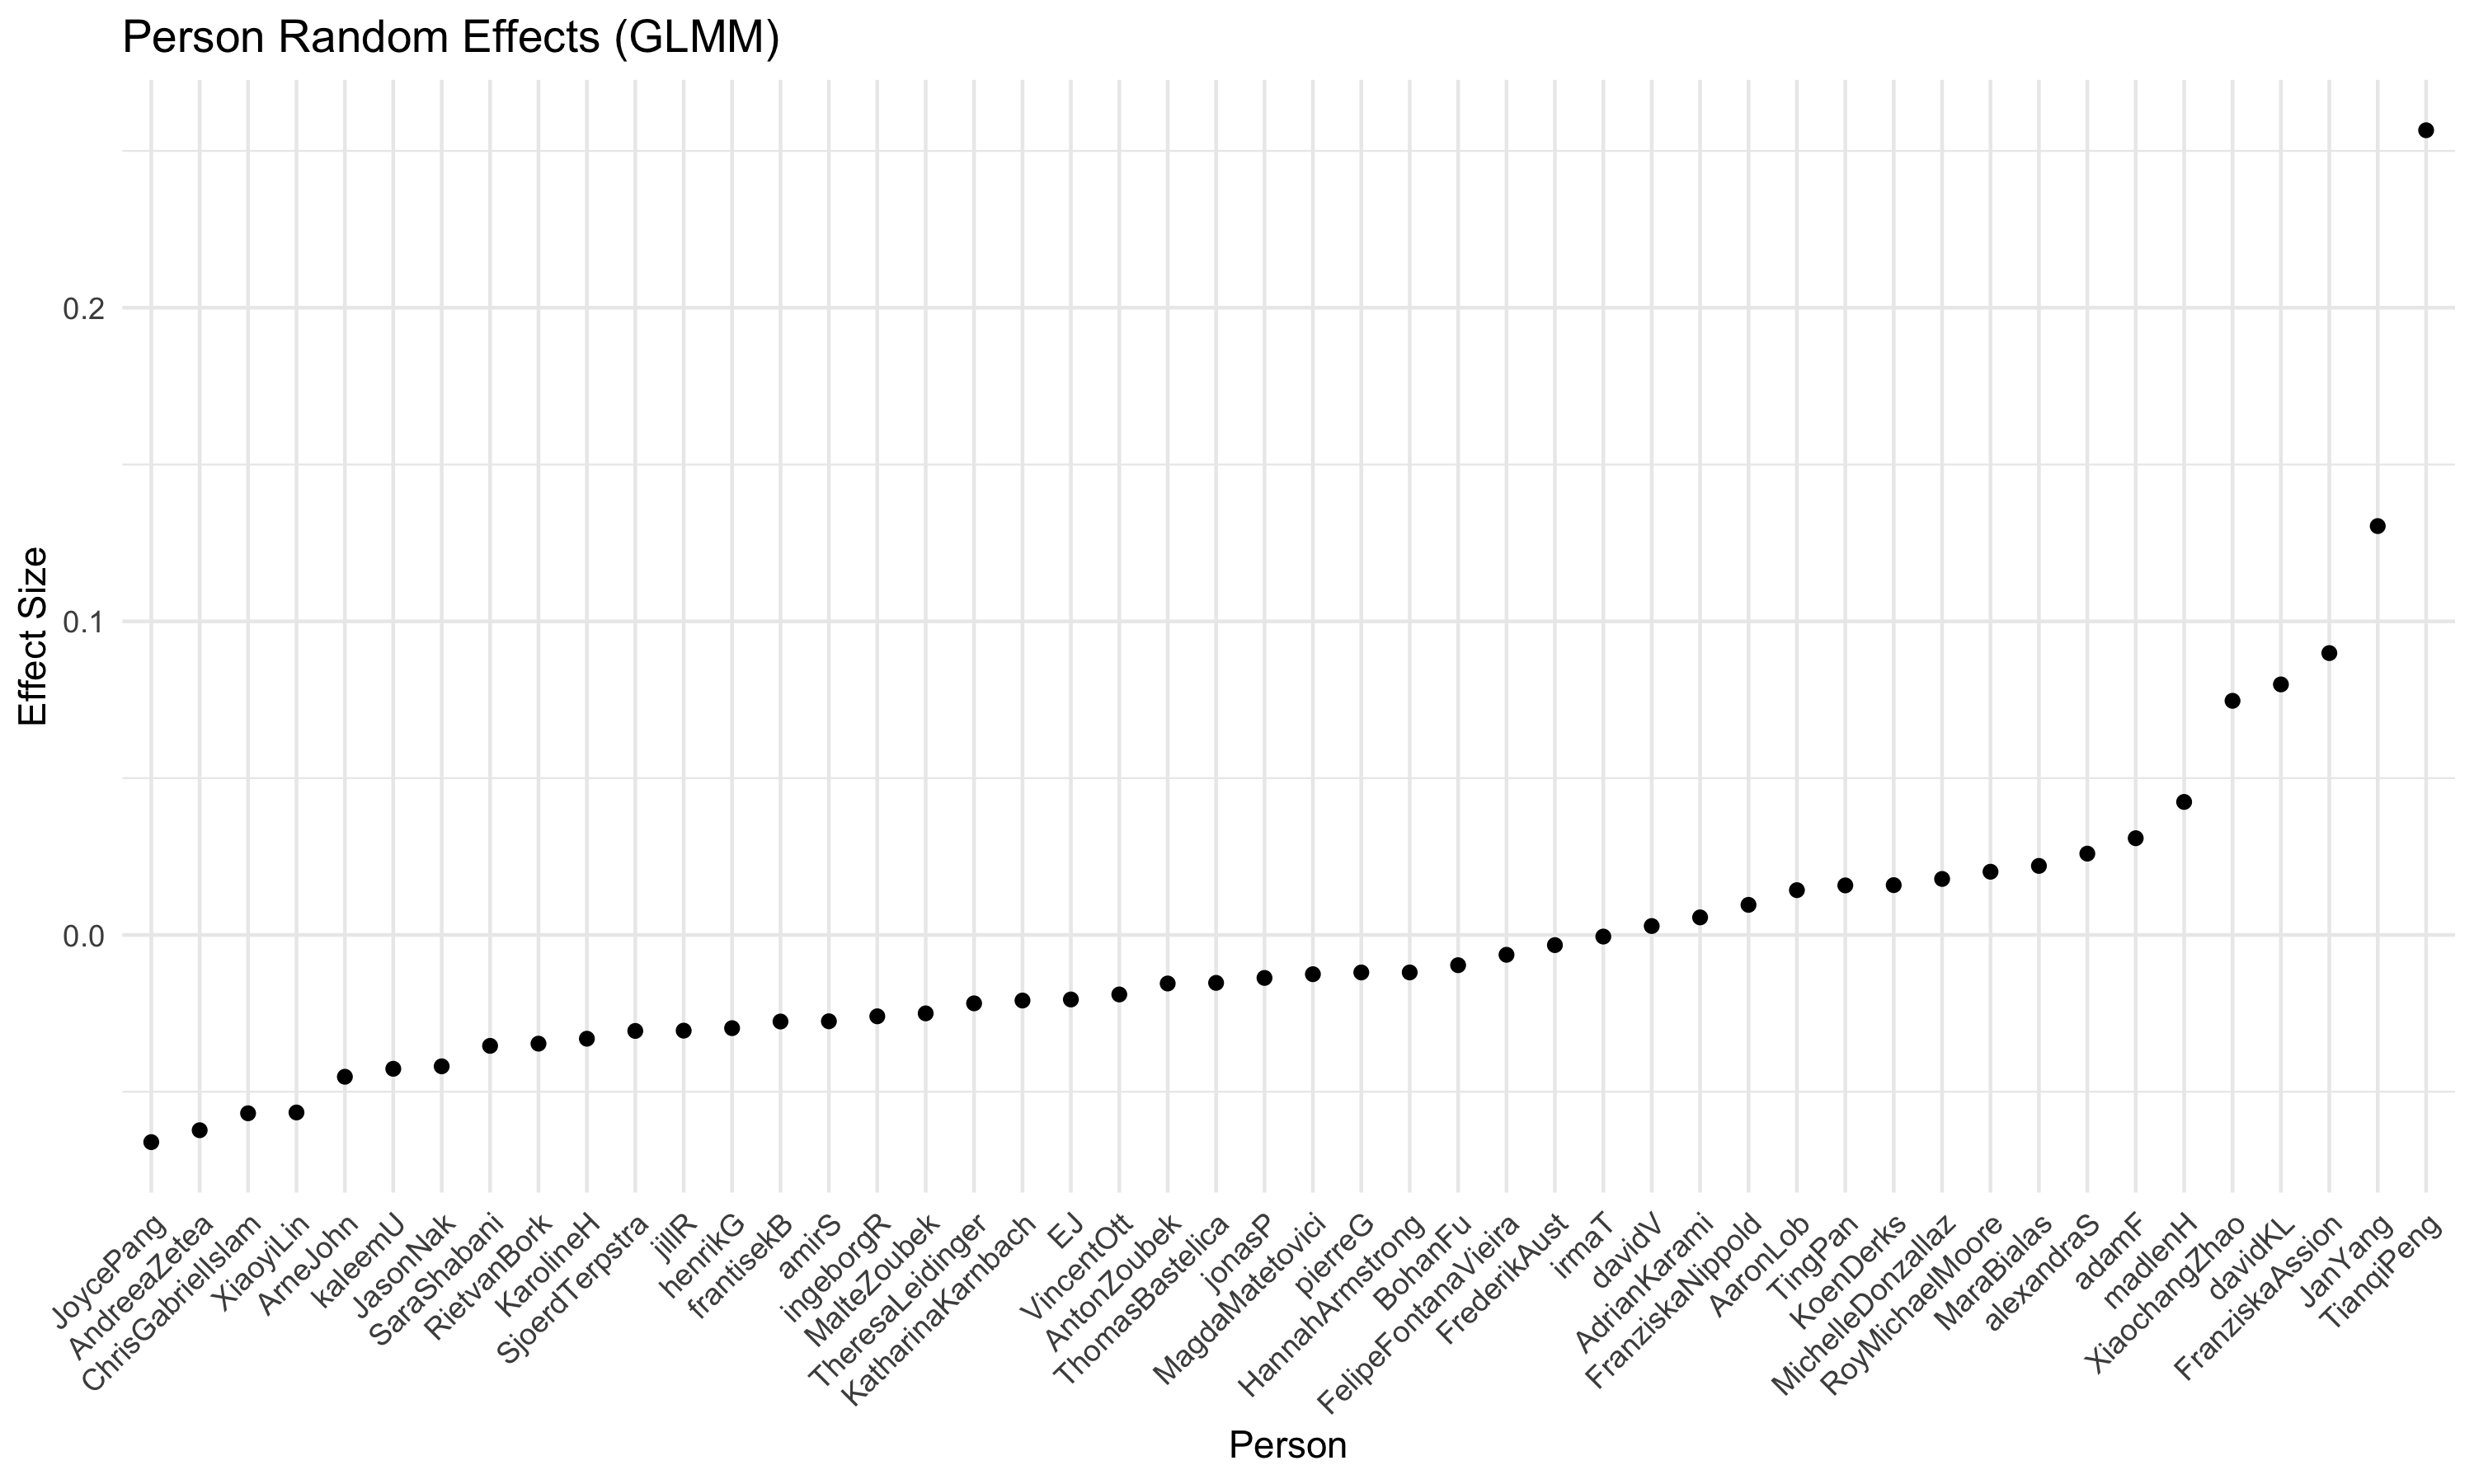
\includegraphics[width=0.8\linewidth]{person_effects_glmm.png}
    \caption{Individual Random Effects from GLMM}
    \label{fig:person-effects}
\end{figure}

The analysis of individual random effects shows:
\begin{itemize}
    \item Most participants' random effects cluster around zero, indicating behavior close to the population average
    \item A few participants show significant deviations, possibly reflecting unique flipping techniques or habits
    \item The effect size range of approximately ±0.2 suggests moderate individual differences
\end{itemize}

\begin{figure}[h!]
    \centering
    \includegraphics[width=0.8\linewidth]{coin_effects_glmm.png}
    \caption{Coin Random Effects from GLMM}
    \label{fig:coin-effects}
\end{figure}

The analysis of coin random effects indicates:
\begin{itemize}
    \item Coin effects show less variability than person effects
    \item Most coins cluster within ±0.1 of the mean effect
    \item A few coins show larger deviations, possibly related to their physical characteristics
\end{itemize}

\subsection{Model Diagnostics}
\begin{figure}[h!]
    \centering
    \includegraphics[width=0.8\linewidth]{model_comparison_plot.png}
    \caption{Model Predictions Comparison}
    \label{fig:model-comparison}
\end{figure}

Model diagnostic results show:
\begin{itemize}
    \item Both models' predictions correlate well with actual values
    \item GLMM performs slightly better at predicting extreme values
    \item Residual analysis shows no obvious systematic bias or heteroscedasticity
\end{itemize}

\section{Discussion}
Based on the results from both modeling approaches, we can draw the following main conclusions:

\begin{itemize}
    \item A significant same-side bias exists, though the effect size is relatively small
    \item Individual differences are the most important factor in explaining data variability
    \item Coin characteristics have a secondary but still significant influence
    \item No significant learning effects were detected
    \item Experimental group effects (bachelor, internet, marathon) are relatively minor
\end{itemize}

These findings suggest that while coin flips are approximately random, there are detectable systematic biases. These biases primarily stem from individual flipping techniques rather than coin characteristics. This has important implications for using coin flips as randomization tools in experimental design.

\bibliographystyle{plain}
\bibliography{references}

\end{document} 